\documentclass{article}
\usepackage[utf8]{inputenc}
\usepackage[style=numeric]{biblatex}
\usepackage[pdftex]{graphicx}

\addbibresource{references.bib}

\title{HERMES: A concept for automated workflows for software publication with rich metadata}
\author{
Druskat, Stephan \texttt{stephan.druskat@dlr.de}\and
Bertuch, Oliver \texttt{o.bertuch@fz-juelich.de}\and
Juckeland, Guido \texttt{g.juckeland@hzdr.de}\and
Knodel, Oliver \texttt{o.knodel@hzdr.de}\and
Schlauch, Tobias \texttt{tobias.schlauch@dlr.de}
% \and (following are comments-only editors exported by SciFlow)
% Mittermaier, Bernhard \texttt{b.mittermaier@fz-juelich.de}
}
\begin{document}
\maketitle


\section{Abstract}\label{sec:abstract}
To satisfy the principles of FAIR software, software sustainability and software citation, research software must be formally published. Publication repositories make this possible, and provide published software versions with unique and persistent identifiers. However, software publication is still a tedious manual process.

To streamline software publication, HERMES, a new project funded under the Helmholtz Metadata Collaboration, develops automated workflows to publish research software with rich metadata.

The tooling developed by the project utilizes continuous integration solutions to retrieve, collate, and process existing metadata in source repositories, and publish them on publication repositories, including checks against existing metadata requirements. To accompany the tooling and enable researchers to easily reuse it, the project also provides comprehensive documentation, and templates for widely used CI solutions. In this paper, we outline the concept for these workflows, and describe how our solution advance the state of the art in research software publication.



\section{Introduction}\label{sec:introduction}
There is increasing awareness that software is a valid research output and should be treated as such \cite{11045035/YUM73BP7}. Thus, software is increasingly published in public repositories or software journals \cite{138880/CVGZJALP}, which is a necessary step in transferring the FAIR principles to software \cite{11045035/FNK2BYH3}, i.e., for finding, understanding, reusing, sharing and citing, and promoting software to first class research citizenship. Recent policy updates (e.g., at Helmholtz Association (HGF) \cite{11045035/N56QGRXT} and funders such as the Deutsche Forschungsgemeinschaft (DFG) \cite{11045035/YMQTEV42}) reflect this progress, and metrics for published software may inform funding decisions in the future.

The main driver for a fulfillment of the functions of FAIR software \cite{138880/DPXVI66D} is software metadata, and thus, publication of research software with rich metadata is essential. In modern research software development, metadata on different software properties is created automatically, semi-automatically or manually at different stages, and in different places and formats. While this metadata can already be collected, verified and validated, and edited to be published with software, there is currently no streamlined, automated process or workflow to do so. This in turn disincentivizes the researchers, research software engineers, and maintainers who create and maintain research software, to publish it with rich metadata.

In this paper, we describe a concept for automated publication of research software with rich metadata via existing automation tools. The concept is being developed in the project HERMES (HElmholtz Rich MEtadata Software Publication), conducted at the German Aerospace Center (DLR), Forschungszentrum Jülich (FZJ) and Helmholtz Zentrum Dresden Rossendorf (HZDR), and funded by the Helmholtz Association of German Research Centers‘ Helmholtz Metadata Collaboration (HMC) initiative (see \ref{giyko1j}).

The work packages related to the concept as described in this document yield a number of outputs: 

\begin{itemize}
  \item software to retrieve existing software metadata in source code repositories, collate and process them to produce a coherent set of metadata for the current state of a given repository;
  \item templates, e.g. for \ref{qo8o3ddicwv8} systems and workflow engines, to run the metadata tools on a user’s source repositories;
  \item documentation and examples for the outputs the project provides.
\end{itemize}

In the following sections, we describe the state of the art for software metadata, available tooling to work with metadata, and existing approaches to automation. We then lay out our concept for research software deposits with rich metadata in automated workflows for two target platforms. In the process, we specify requirements for the structure and contents of source code repositories, define an iterative process for the inclusion of increasingly unstructured metadata, detail the scope of the project, and provide a high-level outline of the implementation of both interfaces and tooling. 

We conclude by requesting feedback from the community on the overall project plan. Based on this document and any feedback we receive, the HERMES project partners design interfaces and develop software tools to automatically aggregate metadata included in software repositories. Taken together, the interfaces and software tools provide an extensible, \ref{qo8o3ddicwv8}-driven serverless solution that enables direct ingestion into publication repositories, such as Zenodo or Harvard Dataverse and other repositories using the underlying InvenioRDM or Dataverse project software. 



\section{State of the art}\label{sec:state-of-the-art}


\subsection{Metadata}\label{sec:metadata}
Software metadata provides information about software, or specific properties of software. It is created intentionally, or generated as a side-product during software development processes. As such, metadata can also pertain to different parts of software, or a software package (\ref{ryblo0s6xdu}) as a whole. Additionally, it can exist in different modes, i.e., as structured or unstructured metadata. It may also pertain to different aspects of the software, e.g., the license regulating its use and development, its creation context, etc. Consequently, there exist different types of metadata.

Software metadata may be provided in a specific form in a dedicated file, or as part of a file, that is part of a software codebase, but it may also be provided in other places, such as in a version control system or another form of repository, in the file system hosting the software source code, or in the system that is running a software package.  

Structured metadata, especially when persisted in files, may furthermore come in a specific format. This format may be a standard format by way of formal standardization or community practice.

In this section, we describe different types of software metadata, as well as formats and standards.



\subsubsection{Types}\label{subsec:metadata-types}
There are generic types of metadata that exist for software but may also be found for other digital data, as well as software-specific metadata. The latter is partly due to the fact that software is both static (as source code, i.e., digital data) and dynamic (at runtime) \cite{138880/U87URNI5}: while software shares some metadata types with other static digital data, a subset of the metadata pertaining specifically to software is bound to the state(s) it passes through when being executed. For this iteration of HERMES, we only focus on software source code metadata - i.e., those pertaining to the static state of software - that is statically available, and is not the product of aggregation or statistical analysis.

Generic software metadata includes:

\begin{itemize}  
  \item Software name
  \item File system metadata (e.g., file sizes, number of files, etc.)
  \item Authorship and contributorship information
  \item Reference to the documentation pertaining to the software
  \item Legal and licensing information
  \item Funding information
  \item Domain context
  \item Citation metrics
  \item Location metadata (e.g., download or instance URLs, etc.)
  \item Publication dates, etc.
  \item Categorization information (e.g., application category, keywords, etc.)
  \item Availability information (purchasing costs, etc.)
  \item Identifiers
  \item Relational metadata (e.g., if the software is part of another work)
  \item High-level description
\end{itemize}

Software-specific metadata includes:

\begin{itemize}  
  \item Dependency information
  \item Lines of code
  \item Programming language
  \item Version information (e.g., metadata from version control systems, publication platforms, or even file names; version identifiers, etc.)
  \item Runtime requirements, including hardware requirements
  \item References to work the software is built on, or relates to
  \item Software metrics (e.g., quality metrics, code coverage, etc.)
  \item Development metrics (e.g., pertaining to bugs/issues, pull/merge requests)
  \item Usage metrics
  \item Infrastructural metadata (e.g., build and CI systems used to produce version artifacts, etc.)
\end{itemize}

\subsubsection{Formats}\label{subsec:metadata-formats}
Some metadata are persisted in files that have specific formats, or are integrated in specific formats as part of other files. Other metadata must be retrieved from third-party systems, e.g., the version control system, source code platform (GitHub, GitLab, or other), etc., if available. Some are only available no other platforms or systems, and may not be retrievable from the source code repository.



\subsubsubsection{Plain text}\label{subsubsec:metadata-formats-plaintext}
Some software metadata is provided in plain text. There are some typical dedicated plain text files, such as license files (LICENSE, etc.) or citation metadata files (plain text CITATION files), that can reasonably be assumed to contain only relevant metadata. Other files mix metadata and other information, such as documentation files (README files and other plain text documentation), community files containing contributor information, a code of conduct, governance information, or other information. Other relevant metadata may be provided in plain text in a less overt manner, e.g., embedded in source code files. 

Generally, while plain text metadata is easily accessible for human readers, they are perhaps the hardest to process using automated approaches. This is due to their less structured form and a lack of clarity with regard to semantics. A plain text CITATION file, for example, may provide retrievable publication metadata, but there is no way of automatically verifying that the metadata unambiguously pertains to a specific version of the software it is provided with, or indeed something else entirely. The same is true for any plain text metadata, and specifically for metadata that are embedded in plain text: While methods exist to extract metadata from plain text, they rely on heuristics that can only produce assumptions with some degree of confidence in their significance and correct categorization.



\subsubsubsection{schema.org}\label{subsubsec:metadata-formats-schema-org}
schema.org\cite{138880/PI4Z5AFK} provides schemas for structured data markup. These are commonly used in HTML to provide metadata that is reused by search engines. schema.org schemas are also used as basis for metadata in RO-Crate\cite{138880/S5F3HZ96}. Additionally, there is ongoing work to align the CodeMeta schema\cite{138880/NBDB4VHJ} with schema.org.



\subsubsubsection{CodeMeta}\label{subsubsec:metadata-formats-codemeta}
CodeMeta \cite{138880/NBDB4VHJ} is a format for generic software metadata, implemented in JSON-LD. It is used to provide comprehensive information about software, with some focus on academic use cases.



\subsubsubsection{Citation File Format}\label{subsubsec:metadata-formats-cff}
The Citation File Format \cite{138880/M4MT8YLA} is a format to provide citation metadata for software, implemented in YAML. Its focus is exclusively to provide citation-relevant metadata in a form that is both human- and machine-readable.



\subsubsubsection{Zenodo JSON}\label{subsubsec:metadata-formats-zenodo-json}
The open access publication platform Zenodo \cite{138880/BG42K9CX} uses its own metadata schema, implemented in JSON. The schema is used in practice to provide metadata for works that are being published on Zenodo, e.g., through the GitHub-Zenodo integration.



\subsubsubsection{BibTeX}\label{subsubsec:metadata-formats-bibtex}
BibTeX files contain citation metadata for one or more works. The format is standardly used as input for citations and bibliographies in LaTeX documents, but is sometimes also adapted to provide citation metadata for software, for example in a dedicated file in source code repositories (sometimes called CITATION), or embedded in a text or marked up document such as a README file. In the context of metadata retrieval, BibTeX files or snippets pose the same challenges as plain text due to their generic nature. It is hard to understand if a BibTeX item is describing the software package it is provided with, one of its versions, or something else entirely.



\subsubsubsection{Manifest files}\label{subsubsec:metadata-formats-manifests}
Manifest files describe a software package or a subunit of a software package. They exist for different programming languages and frameworks, and come in a variety of implementation formats. Some examples include Project Object Model (POM) XML files for Java projects using the Apache Maven build management tool, JAR manifests for packaged Java applications, or setup.py/pyproject.toml files that contain metadata for Python packages built with Python’s distutils.



\subsubsubsection{Configuration files}\label{subsubsec:metadata-formats-config}
Configuration files are often added to source code repositories to leverage third-party tools such as continuous integration services or source code or documentation generators. They come in different formats, of which common ones are plaintext key-value, INI, TOML, YAML, JSON and XML. Configuration files may include metadata pertaining to, e.g., software dependencies, development and publication processes, etc. One popular example for configuration files that contain contribution metadata are those for the All Contributors specification.



\subsubsubsection{Linked Data}\label{subsubsec:metadata-formats-linked-data}
Linked data provides an extensible way to describe research software in depth. Common linked data formats are based on RDF \cite{11045035/RZXJXX75}, using serializations like JSON-LD \cite{11045035/DQRH6UQP} or Turtle \cite{11045035/F3ARKWX4}. They express not just attributes or simple relations, but by reusing formalized concepts (ontologies) they may describe usage, ideas, context, etc., in much greater depth than other formats listed above.

Although ontologies are a powerful concept, there does not seem to be sufficient uptake of using software ontologies to describe software in practice. This may change in the future.

Commonly known ontologies for software include \cite{11045035/TVVPYY5L}, \cite{11045035/5JK345NF}, \cite{11045035/A8V7DJ4R} and \cite{11045035/YPMVLAM4}.



\subsubsubsection{Platform API responses}\label{subsubsec:metadata-formats-apis}
While not strictly a format, software metadata is also available from different (e.g., REST) APIs, such as those for querying software development platforms such as GitHub or GitLab, WikiData, or publication repositories. These may provide metadata on software development processes, version control, contributions, publications, and other metadata. These APIs can usually be queried through their endpoints, or globally using a common query language such as \cite{138880/D5YC8HI5}, and responses are usually provided as JSON or XML that can easily be persisted and reused.



\subsubsection{Comparison of formats metadata type capabilities}\label{ic5kiajfpf04}
Table \ref{y2o46dfd3ike} shows a mapping of metadata types to the formats they are commonly provided in.

\begin{figure}
\begin{tabular}{lllllllllll}


& Plain text

& CodeMeta

& Citation File Format

& Zenodo JSON

& BibTeX

& Manifest files

& Configuration files

& Platform APIs

& Linked Data

& Other

\\
Software name

& x

& x

& x

& x

& x

& x

& 

& x

& x

& 

\\
File system metadata

& 

& 

& 

& 

& 

& 

& 

& 

& x

& x

\\
Authorship information

& x

& x

& x

& x

& x

& (x)

& (x)

& (x)

& x

& 

\\
Documentation reference

& x

& x

& 

& 

& 

& 

& x

& x

& x

& x

\\
Legal and licensing information

& x

& x

& x

& x

& 

& x

& 

& x

& x

& x

\\
Funding information

& x

& x

& 

& x

& 

& 

& 

& 

& x

& x

\\
Domain context

& x

& 

& 

& 

& 

& (x)

& 

& (x)

& x

& x

\\
Citation metrics

& x

& 

& 

& 

& 

& 

& 

& x

& x

& x

\\
Location metadata

& x

& x

& x

& 

& (x)

& 

& (x)

& x

& x

& x

\\
Publication dates, etc.

& 

& x

& x

& x

& x

& 

& 

& x

& x

& 

\\
Categorization information

& x

& x

& x

& x

& 

& (x)

& 

& (x)

& x

& x

\\
Availability information

& x

& 

& 

& 

& 

& 

& 

& 

& x

& x

\\
Identifiers

& x

& x

& x

& x

& x

& 

& 

& (x)

& x

& x

\\
Relational metadata

& x

& x

& 

& x

& 

& x

& 

& (x)

& x

& 

\\
High-level description

& x

& x

& x

& x

& (x)

& (x)

& 

& (x)

& x

& 

\\
Dependency information

& x

& (x)

& x

& 

& 

& x

& (x)

& (x)

& x

& 

\\
Lines of code

& 

& 

& 

& 

& 

& 

& 

& x

& x

& x

\\
Programming language

& x

& x

& 

& 

& 

& x

& x

& x

& x

& 

\\
Version information

& x

& x

& x

& x

& (x)

& x

& (x)

& x

& x

& x

\\
Runtime requirements

& x

& x

& 

& 

& 

& x

& x

& 

& x

& x

\\
References

& x

& (x)

& x

& x

& 

& x

& (x)

& x

& x

& x

\\
Software quality metrics

& x

& 

& 

& 

& 

& 

& x

& x

& x

& x

\\
Development metrics

& x

& 

& 

& 

& 

& 

& 

& x

& x

& x

\\
Usage metrics

& x

& 

& 

& 

& 

& 

& 

& x

& x

& x

\\
Infrastructural metadata

& x

& (x)

& 

& 

& 

& 

& x

& x

& x

& x

\\
\end{tabular}
\caption{Mapping metadata types to common metadata formats.}
\label{y2o46dfd3ike}
\end{figure}

\subsection{Standards}\label{subsec:metadata-standards}
As of now, there are no software metadata formats relating to our work that are formally standardized and cover HERMES’ scope completely. Some de facto standards exist. CodeMeta’s ongoing alignment with schema.org is a promising path to at least de facto standardization. The DataCite Metadata Schema \cite{138880/AJSS9RWC}, although used widely, has a much more generic scope again than, e.g., CodeMeta, and does not implement as large a vocabulary pertaining to software (see the CodeMeta-DataCite crosswalk).

Standards in similar stages exist in related areas, such as for research objects in general: RO-Crate \cite{138880/S5F3HZ96} packages research objects with their metadata, with a metadata schema based on schema.org. BagIt \cite{138880/CE9VUDMM} is a generic packaging standard used in, e.g., libraries, to package file structures with metadata, where the metadata schema is very generic and not targeted to software specifically.



\subsection{Integrations}\label{subsec:metadata-integrations}
Some platforms and tools provide integrations for some of the above-mentioned formats. As opposed to concrete (software) tools for working with formats that are available to end-users, integrations are embedded in their hosts and are not directly addressable by users.

Plain text. Many platforms support metadata provided in plain text or lightweight markup languages by rendering them for presentation to end users. This often includes detecting URLs and converting them to HTML hyperlinks. Examples include Markdown rendering on, e.g., GitHub, GitLab, and many other platforms.

schema.org.

\begin{itemize}  
\item  RO-Crate uses schema.org schemas to record and provide core metadata.


\end{itemize}CodeMeta 

\begin{itemize}  
\item Software Heritage uses a subset of the CodeMeta vocabulary to map intrinsic metadata formats discovered in source repositories.


\item CaltechDATA ingests CodeMeta files to create metadata records from the included metadata.


\item The Astrophysics Source Code Library (ASCL) produces pre-filled CodeMeta files from its records. This functionality is accessible to users through appending the URL for a record page with ‘/codemeta.json’.


\end{itemize}Citation File Format 

\begin{itemize}  
\item Via its Github-Zenodo integration, Zenodo ingests the metadata from CITATION.cff files and uses them to populate their metadata records.


\item Via its connector browser plugins, Zotero ingests CITATION.cff files discovered in source code repositories and saves the metadata in its internal format. 


\item JabRef can import CITATION.cff files (feature merged, currently awaiting release). 


\item The Astrophysics Source Code Library (ASCL) produces pre-filled CITATION.cff files from its records. This functionality is accessible to users through appending the URL for a record page with ‘/CITATION.cff’. 


\item GitHub provides a template for creating new CITATION.cff files via its UI and ingests existing CITATION.cff files, extracts the metadata, converts them to a citation style and BibTeX, and provides them in a widget for end users to copy.


\item There is ongoing work to implement the same for GitLab.


\item An extension to the Sphinx platform for documentation rendering ingests an existing CITATION.cff file and, converts it to different citation formats, and provides it to end users in a widget for copying (see example).


\item Software Heritage can ingest CITATION.cff as intrinsic metadata format and map it.


\end{itemize}Zenodo JSON 

\begin{itemize}  
\item Via its GitHub-Zenodo integration, Zenodo ingests .zenodo.json files and populates metadata records from the provided metadata.


\end{itemize}BibTeX 

\begin{itemize}  
\item BibTeX is supported by the LaTeX document preparation system and many platforms for creating, editing, converting and rendering LaTeX projects. Usually, the metadata from BibTeX .bib files are converted into string formatted in a citation style and displayed as citations and items in the references list.


\item biblatex-software\cite{138880/DXRLT553} is a reference biblatex implementation of a bibliography style extension that includes software-specific BibTeX entries and integrates these metadata in LaTeX documents via the biblatex implementation for reference management.


\end{itemize}Manifest files 

\begin{itemize}  
\item Some or all information from manifest files is rendered on package/artifact repositories’ sites for the respective package, e.g., on Maven Central Repository, PyPI, etc.


\end{itemize}

\section{Tooling}\label{sec:tooling}
The following section is an attempt to gather tools available for metadata extraction and collection as well as building (automatable) workflows around software depositions.

These lists may not necessarily be complete. Please add new items upon discovery. 



\subsection{Metadata}\label{subsec:tooling-metadata}
Existing toolsets for metadata may operate on different stages of metadata presence.

The spectrum starts at zero prior information and requires extraction from arbitrary text files and context information. Moreover, it can be accomplished by reusing software package metadata via so called crosswalks, or even  conversions between different metadata formats. Some may give users a hand to create well-structured metadata from the start.



\subsubsection{Software Metadata Extraction Framework (SOMEF)}\label{qz3d8r3z48k}
Starting from zero, SOMEF \cite{11045035/AWIJVT4K} \cite{11045035/E5BAXQ4Y} extracts data from README text files and other files that may include metadata using a neural network. It may also retrieve details from software development platforms such as GitHub, using their APIs. It creates, e.g., CodeMeta JSON-LD or Turtle RDF files using “The Software Ontology” \cite{11045035/TVVPYY5L}. It is an active software project \ref{msegj6m7qry}.



\subsubsection{CaltechDATA Automated Metadata Service (AMES)}\label{v9uri13hoesk}
AMES \cite{11045035/CBYX26KG} may be used to create and update scholarly output records in services like CaltechDATA, highly specific for Caltech and based on \ref{vym1mq9h5jxs}. For software publications a Python script to update \ref{vym1mq9h5jxs} records from \ref{subsubsec:metadata-formats-codemeta} files is in use\footnote{See also https://github.com/ASCLnet/SWRegistryWorkshop/blob/2cd02ad1862ebc67ad9fcb0347b832d10d8c7ca9/presentations/Caltech-Software-Presentation.pptx}.. It is an active software project \ref{msegj6m7qry}.



\subsubsection{codemeta2cff GitHub Action}\label{tk14z3o75c5t}
The codemeta2cff GitHub Action\cite{138880/U54AXTI4} provides automatic conversion from a CodeMeta file to a Citation File Format file in a GitHub Action.

It is an active software project \ref{msegj6m7qry}.



\subsubsection{CodeMeta Crosswalks}\label{ks3fezwj69ji}
CodeMeta Crosswalks \cite{11045035/2G9VU24E} are a set of comma separated value (CSV) files, containing two columns. Each row depicts a metadata field in CodeMeta and a corresponding field in some other schema. While not an executable tool, these crosswalks describe a mapping with limited interoperability, as most other standards aren’t as detailed.

It is an active software project \ref{msegj6m7qry}.



\subsubsection{CodeMeta Generator}\label{vuql4sg8sy2}
CodeMeta Generator \cite{11045035/BGVLLAZ8} is a Javascript-based web UI to help you create a CodeMeta file for inclusion in your software repository. It is an inactive software project \ref{msegj6m7qry}.



\subsubsection{Citation File Format Converter}\label{dfofurxomlo4}
cffconvert \cite{11045035/3EAAUM9S} is a Python based command line tool to transform a given Citation File Format  file into other destination formats like Bibtex \ref{subsubsec:metadata-formats-bibtex}, CodeMeta \ref{subsubsec:metadata-formats-codemeta} and others. It is an active software project \ref{msegj6m7qry}.



\subsubsection{Citation File Format Initializer}\label{bv2fu3l3kcxk}
cffinit \cite{11045035/244Q39FZ} is a Javascript based interactive web form to assist you in creating a new or updating an existing CFF \ref{subsubsec:metadata-formats-cff} file in your browser. It is an active software project \ref{msegj6m7qry}.



\subsection{Workflows}\label{w6t3wd4fqysc}
The following tools provide building blocks to create an automatable depositing workflow, interfacing with target repositories, registries or archives.



\subsubsection{Zenodraft}\label{o71h0jljbmme}
Zenodraft \cite{11045035/VXRILTTG} may be used to draft, push and publish new deposits on Zenodo, a commonly known general purpose repository based on Invenio RDM \ref{vym1mq9h5jxs}.

New and existing deposits may be enhanced with metadata via Zenodo JSON \ref{subsubsec:metadata-formats-zenodo-json} files.

It is a WIP software project \ref{msegj6m7qry}.



\subsubsection{Software Heritage Github Action}\label{tzwlyl3ildzb}
SWH Github Action \cite{11045035/U5SGIYLE} acts like a webhook: it sends a archive request to an Software Heritage Archive API endpoint with the repository to archive given as parameter.

Software Heritage Archive services take care of reading a codemeta.json \ref{subsubsec:metadata-formats-codemeta} or CITATION.cff \cite{138880/M4MT8YLA} file (if included) to add metadata to its archive.

It is a WIP software project \ref{msegj6m7qry}.



\subsubsection{Software Heritage Deposit Command Line Tool}\label{k8b3f8dzavl}
The CLI part of a SWORD \cite{138880/5XMKCCSZ} based deposition service for the Software Heritage Archive may be used to actively push metadata and/or artifact ingests. It seems not to be intended for public usage but integrations with software/data repositories.



\subsection{Publication repositories}\label{px3vrgozgpce}
Publication repositories \ref{bu8qxagwu08b} are public catalogues containing publications of digital artifacts together with the metadata describing them. Usually, publication repositories provide landing pages for each artifact, including versions of the same object. As such, they are different from registries, that usually focus on the collection of metadata and their presentation. They are also different from archives, that focus on long-term archival of artifacts only. Additionally there may exist differences in how records are added to publication repositories, registries and archives.

One of the main advantages of publication repositories is that they enable a combination of discovery of digital objects through their metadata, and direct access to the object artifacts themselves. HERMES focuses on publication repositories exclusively, and specifically on two publication repository software projects as deposition targets, for the reason that they represent commonly used platforms both within the Helmholtz Association and beyond: Dataverse and InvenioRDM.

Research software is also represented in digital preservation archives, catalogues and directories. Targeting these platforms may be a future direction of development for HERMES, see also \ref{owiy885c2loj}.



\subsubsection{Dataverse Project}\label{adb4j1s8jlul}
The Dataverse Project is an open source repository software.

Its focus is currently on providing services for data deposition, although software may be deposited as part of datasets, too. No builtin support for software metadata schemas, software licenses or propagating software metadata to PID registrars is available.

Despite versioning support for datasets, neither integrating software release versioning is available nor support for software citations as a concept and individual releases.

The Dataverse community runs a working group for software and workflow related topics. Its website can be found at https://swc.wgs.gdcc.io

It is an active software project \ref{msegj6m7qry}.



\subsubsection{InvenioRDM}\label{vym1mq9h5jxs}
The InvenioRDM Project has the goal to provide a turn-key research data management repository based on Invenio Framework and Zenodo. The publication of special software datasets is possible, but the standard set of metadata for the description of Invenio records is used as well as in \ref{subsubsec:metadata-formats-zenodo-json}.

Invenio provides versioning, DOI registration and supports multiple data types for the publication such as Publication, Poster, Presentation, Dataset, Image, Video/Audio, Software, Lesson, Physical objects or Other (List taken from Zenodo). No builtin support for software metadata schemas is available at the moment. 

For a software publication the use of optional webhooks can be used as introduced in \ref{dttj6h7jn6f}.

It is an active software project \ref{msegj6m7qry}.



\section{Workflows}\label{bq4pinu53a8}
The following lists may not complete. If you discover new items that should be included, please let us know via the process for providing \ref{yec0wia}.



\subsection{Pull-based workflows}\label{dttj6h7jn6f}
“Harvesting” for new or changed datasets is an often used pattern within the world of text and data publications. The well-known OAI-PMH is used for inter-repository talk, while harvesting in the context of workflows is attached to pulling from public version control systems like Git.

Using a “webhook” to trigger some action is well known in distributed systems. Within the publication business a “webhook” may trigger a harvesting action with certain parameters like a target.

\begin{figure}
\begin{tabular}{*5{l}}
Tool name

& Type

& Status \ref{msegj6m7qry}

& Supported Formats

& Docs Links

\\
GitHub Zenodo Bridge

& Webhook

& Active

& Zenodo JSON \ref{subsubsec:metadata-formats-zenodo-json}

& https://guides.github.com/activities/citable-code

https://developers.zenodo.org/\#add-metadata-to-your-github-repository-release

\\
Official Gitlab Zenodo Bridge

& Webhook

& Concept

& (presumably same as GitHub)

& https://github.com/zenodo/zenodo/issues/1404

https://gitlab.com/gitlab-org/gitlab/-/issues/25587

\\
RODARE Gitlab InvenioRDM Bridge

& Webhook

& Suspended

& Zenodo JSON \ref{subsubsec:metadata-formats-zenodo-json}

& https://gitlab.hzdr.de/rodare/invenio-gitlab

\\
CaltechDATA AMES \ref{v9uri13hoesk}

& Webhooks

& Active

& CodeMeta \ref{subsubsec:metadata-formats-codemeta}

& See \cite{11045035/44KEF4EY}

\\
Software Heritage Archive

& Harvest

& Active

& CodeMeta \ref{subsubsec:metadata-formats-codemeta}, plus crosswalks \ref{ks3fezwj69ji}

& https://archive.softwareheritage.org/save, \cite{11045035/7EDI2C4A}, \cite{11045035/FYSTKDUI}

\\
SWH Github Action

& CI based Webhook

& WIP

& See above

& See 

\ref{tzwlyl3ildzb}

\\
\end{tabular}
\caption{Pull-based workflow examples}
\label{dououxj84y9j}
\end{figure}

\subsection{Push-based workflows}\label{ogbzdahy00bw}
While pull-based workflow have their advantages, in some scenarios you might want to publish your software in a more active fashion.

Push-based workflows gather metadata and/or artifacts and deposit them via some API endpoint into a service like a repository, registry or archive. They may also split certain tasks across different services, which may be harder to achieve with common pull-based workflows.

Examples for push-based workflows are even harder to find than pull-based workflow approaches. This might be due to the convenience of commonly known pull-based workflows and the not-yet popular task of software publications. Please let us know of any example we haven’t listed yet.

\begin{figure}
\begin{tabular}{*5{l}}
Tool name

& Type

& Status\ref{msegj6m7qry}

& Supported formats

& Links

\\
SARA

& Web application

& Unsupported

& Bespoke?

& See \cite{138880/UM3ZH6ZQ}, https://www.sara-service.org/

\\
OpenCARP CI

& Automatable scripts for releasing, archiving, website generation

& Active

& GitLab API, DataCite Metadata, custom YAML, BagIT, BagPack, Markdown, BibTeX, Python dosctrings

& https://git.opencarp.org/openCARP/openCARP-CI

\\
Zenodraft

& CLI, GitHub Action

& Active

& Zenodo deposit (Zenodo JSON), CITATION.cff

& See \cite{138880/KWIHDXNN}, https://github.com/zenodraft, usage example: https://github.com/citation-file-format/cff-initializer-javascript/blob/main/.github/workflows/zenodraft.yml

\\
PresQT

& Web application

& Unsupported

& BagIT, OSF API, GitHub API, GitLab API, Zenodo API, Figshare API

& https://presqt.crc.nd.edu/

\\
\end{tabular}
\caption{Push-based workflow examples}
\label{txalpo9fsoli}
\end{figure}

\section{The HERMES concept for automated workflows for rich metadata software publication}\label{az624rg}


\section{Overview}\label{qdsioybmcwum}
The coupling of software development platforms with publication repositories for automated data exchange is a first and important step for easier and automated software publications. This technical foundation also immediately raises the question as to the requirements towards a source code repository on a development platform to benefit from such automation. Current first generation tools simply copy the content of a source code repository to create or update a publication repository entry. The metadata of the publication repository entry can originate from a special file in the source code repository.

Questions addressed by HERMES that extend the status quo are:

\begin{itemize}  
\item How to treat different components in a source code repository (actual software, documentation and data)?


\item How to deal with source code repositories that contain more than one software product?


\item How to deal with publication of directly executable software artefacts generated from the software repositories?


\item How to enabled closed source but FAIR software\cite{138880/DPXVI66D} for these processes?


\end{itemize}

\section{Source code repositories}\label{kocqhrfewb2}
HERMES targets both GitHub and GitLab as software development platforms as they are the de facto community standard and are widely used both as public cloud services and on-premise installations. Both services offer an API for interaction with other services and, thus, provide an ideal starting point for HERMES to add on to the existing solutions.



\subsection{Different ways of setting up software projects}\label{c06sju9is784r}
A source code repository containing only one software package is an easy, common case and straightforward in publication. Integrated software documentation as part of the repository is considered a part of the software package and does not need to be treated differently.

For other cases, e.g., data alongside the source code or multiple software packages in one source code repository, HERMES provides methods for the user to specify which parts of the repository to include in a publication.



\section{Metadata sources}\label{s43q35fgxc42}
HERMES decidedly does not limit the metadata sources it works on to specific types. However, implementation follows an iterative process, with support for different types being added in stages.

\begin{enumerate}  
\item Firstly, we collect structured metadata that can be tested for availability, e.g., dedicated metadata files, such as codemeta.json, CITATION.cff, LICENSE files, Version control metadata, software development platform metadata.

\item Secondly, we attempt to mine structured data that may or may not contain relevant metadata, e.g., manifest files, configuration files, etc.

\item Finally, we attempt to mine unstructured metadata from, e.g., plain text files.


\end{enumerate}

\section{Scope}\label{g3qi39vk1lgb}
HERMES aims to enable software publications in publication repositories where metadata is transported from the source code repository to the publication repository. During this first iteration of the project, HERMES interfaces with two popular publication repository software products: Dataverse project \ref{adb4j1s8jlul} and InvenioRDM \ref{vym1mq9h5jxs}.



\subsection{Out of scope}\label{ak94twwc5mfr}
The tooling developed and provided by HERMES needs to be shaped in scope and size. Thus, at this stage HERMES does

\begin{itemize}  
\item not offer license compatibility checks,


\item not resolve values from external vocabularies (e.g., WikiData, triplestores using software metadata ontologies) or other persistently identified resources (ORCID, ROR, other publications, …),


\item not validate metadata beyond pure linting functionality,


\item not create provenance, workflow or pipeline models (but may be a part of these) and


\item not search or resolve publications of (software) dependencies.


\end{itemize}The software and reusable workflow templates that HERMES provides does not constitute, or be provided as, a “service” (web service, REST API, SaaS, PaaS, IaaS, etc.) or other infrastructure component. Instead, research software projects can reuse the solutions in their own software projects, e.g., by defining their own \ref{qo8o3ddicwv8} workflows based on provided templates. This way, our outputs also have a greater potential of becoming sustainable: once they are persistently distributed, no continuous funding for HERMES is needed to use them. Instead, the community may apply further funding as needed, e.g., for further development.



\subsection{Expectations on users and sources}\label{l24mfxuds6zt}
HERMES cannot clean up messy projects for users. Instead all tooling relies on the user to provide

\begin{itemize}  
\item well-structured source code repositories


\item with separated artifacts for data and software and


\item with any possible legal issues resolved beforehand and appropriatly chosen licenses.


\end{itemize}Additionally, we rely on users to supply any authentication credentials needed for workflows to run successfully. Examples include target publication repositories APIs source code platform APIs, continuous integration systems and the like. 



\subsection{In scope}\label{ir8q16h2mxws}
The user receives assistance in depositing software in an automated fashion. This may be used to create publications purely with rich metadata (to be at least FAIR \cite{11045035/FNK2BYH3}) or with attached artifacts like source code, executables, etc. (to be more easily reusable). To achieve this, HERMES provides

\begin{itemize}  
\item an extensible, configurable and automatable toolchain with capability to be executed for 

\begin{itemize}  
\item N software publications in 


\item M target publication repositories 


\item from the same origin


\item as configured by the user,


\end{itemize}
\item initially harvesting and collating metadata from the sources described in \ref{s43q35fgxc42} and


\item initially targeting (popular within Helmholtz Association)

\begin{itemize}  
\item InvenioRDM \ref{vym1mq9h5jxs} and


\item Dataverse project \ref{adb4j1s8jlul}


\end{itemize}
\item for deposits of metadata and artifacts according to curator-defined institutional requirements


\item and output of the respective metadata in a structured format (e.g., CodeMeta) for further reuse.


\end{itemize}

\subsection{Future scopes and extensions}\label{owiy885c2loj}
In the future HERMES’ extensible architecture can be used to also support archives, such as Software Heritage, and domain and other registries such as ASCL, the Research Software Directory, etc.



\section{Implementation}\label{d9jafc0bwx8g}
As discussed in \ref{ak94twwc5mfr}, we provide metadata tooling and templates to integrate this tooling in automated (\ref{qo8o3ddicwv8}) workflows. In this section, we briefly describe the basic concepts for the implementation of this tooling.



\subsection{Architecture}\label{ichz44bq6tfo}
As described within \ref{g3qi39vk1lgb}, our implementation reuses existing computing resources by leveraging workflows on them. The following figure \ref{uvwszplpisk} uses a C4 Component diagram to outline the overall architecture of our solution.

\begin{figure}
\centering
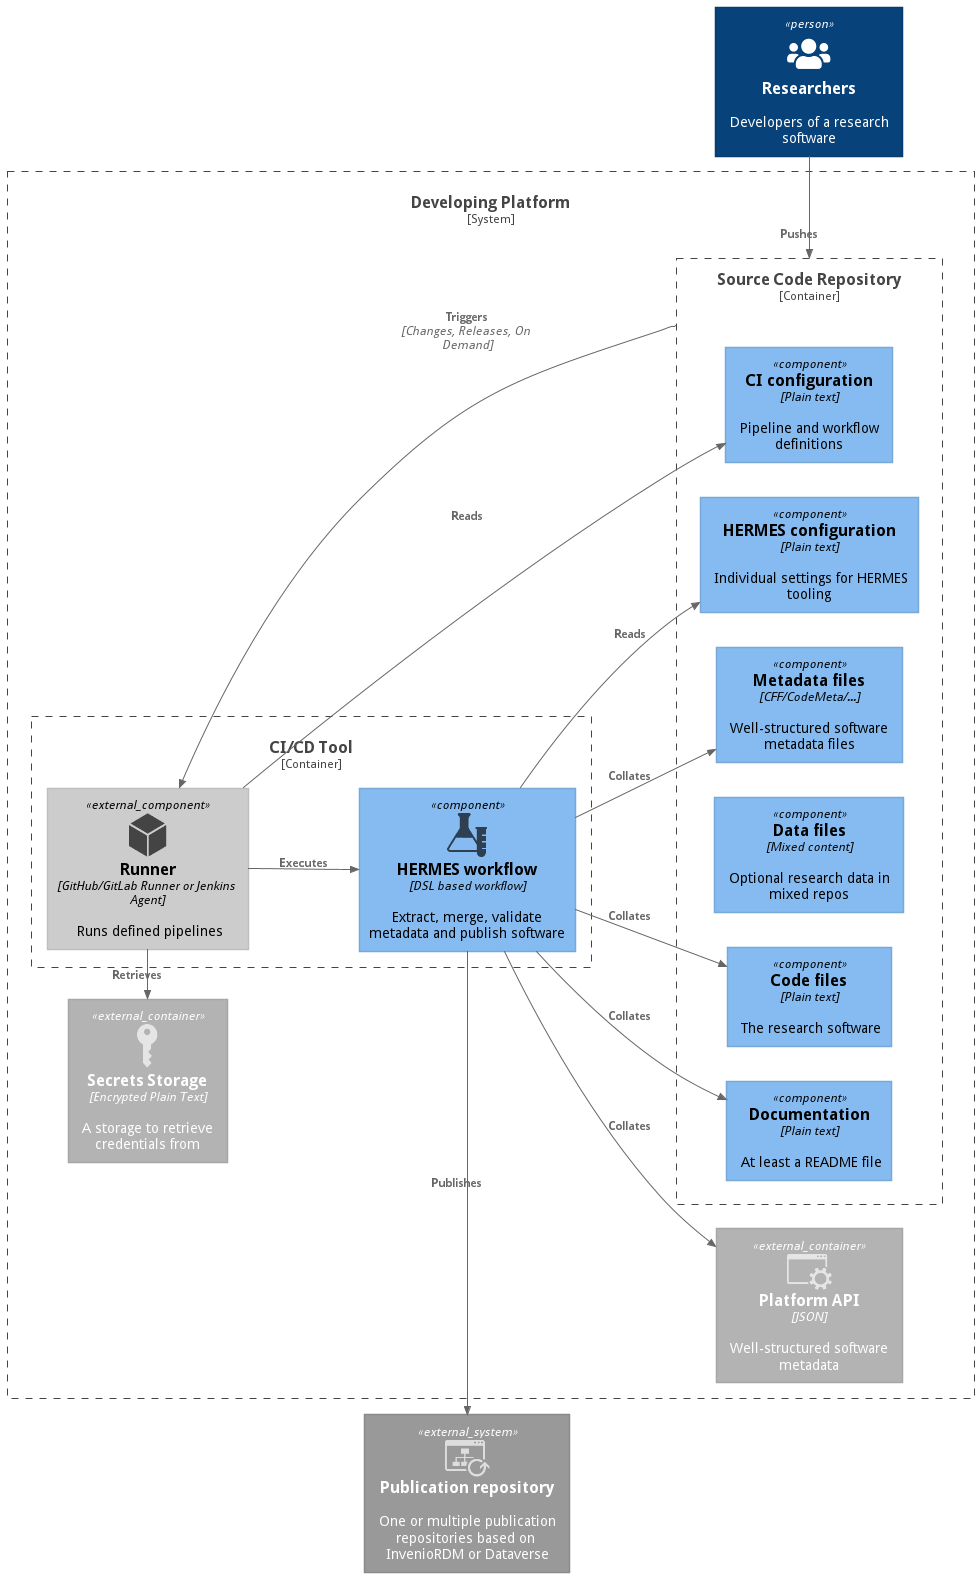
\includegraphics[width=\textwidth]{assets/uvwszplpisk.png}
\caption{C4 Component architecture diagram}
\label{uvwszplpisk}
\end{figure}
It outlines how the HERMES workflow relates to researchers, gets embedded in\ref{qo8o3ddicwv8} runners, collates metadata from sources and publishes in target publication repositories.

\subsection{Workflow pipeline modeling}\label{d6s9gv9l0w6e}
\begin{figure}
\centering
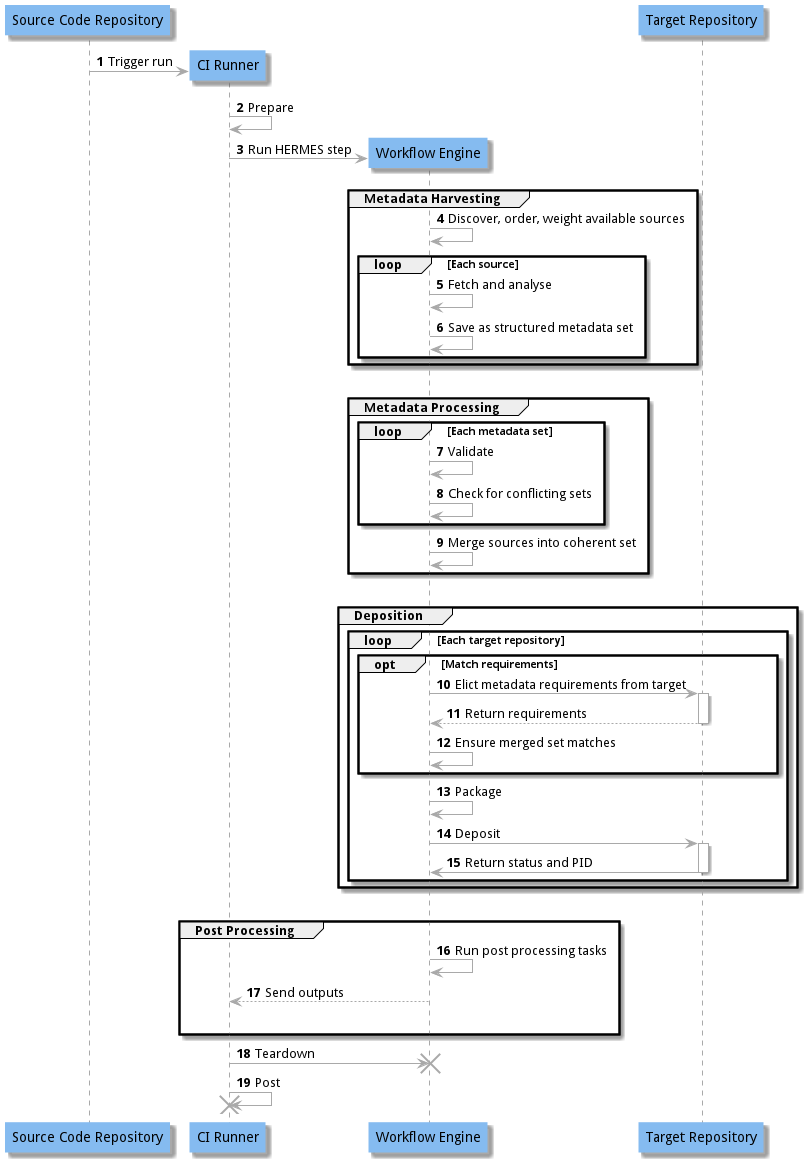
\includegraphics[width=\textwidth]{assets/j4ecrtn7gls3.png}
\caption{Sequence diagram of HERMES workflow pipelines}
\label{j4ecrtn7gls3}
\end{figure}
Simple use case (1 software, n targets) data flow, showing how HERMES workflow pipelines kick into action. Outputs of any pipeline are forwarded to the next pipeline. Both \ref{qo8o3ddicwv8} configuration and pipelines allow for easy modifications or extensions if necessary.As figure \ref{j4ecrtn7gls3} outlines, HERMES implements four discrete pipelines with public interfaces for extensibility and based on existing state-of-the-art \ref{sec:tooling} where possible, namely

\begin{enumerate}  
\item a metadata harvesting pipeline that

\begin{itemize}  
\item runs a metadata analysis to determine the concrete harvesting tools to apply to the discovered \ref{s43q35fgxc42}, and


\item retrieves the existing metadata from \ref{s43q35fgxc42};


\end{itemize}\item a metadata processing pipeline that

\begin{itemize}  
\item validates the retrieved metadata, i.e., checks for conflicting sources, and


\item merges them into a coherent set;


\end{itemize}\item a metadata deposition pipeline that

\begin{itemize}  
\item optionally elicits metadata requirements from target \ref{px3vrgozgpce} and matches the merged set against them,


\item publishes the set of metadata with or without the respective software artifacts to those target repositories, and


\item retrieves the persistent identifier for the deposition; and


\end{itemize}\item a post-processing pipeline that 

\begin{itemize}  
\item optionally updates metadata in the source repositories, e.g., with the deposition identifier,


\item notifies users of any issues that were encountered during the workflow run, and


\item passes the software and deposit metadata to any following steps in the users’ \ref{qo8o3ddicwv8} workflow.


\end{itemize}
\end{enumerate}We also provide reference implementations for commonly used continuous integration tools, such as GitLab CI, GitHub Actions and Jenkins that combine the four pipelines into a complete solution for automated publication of software with rich metadata (see also \ref{ichz44bq6tfo}).



\subsection{Adding missing functionalities to target repository software}\label{hdbbjo6li8d6}
To enable the metadata deposition pipeline described above to publish software with rich metadata, the two targeted publication repositories need to be prepared to accept metadata sets compiled in the metadata processing pipeline.

Both the Dataverse project \ref{adb4j1s8jlul} and InvenioRDM \ref{vym1mq9h5jxs} lack some features for advanced software metadata intake and presentation. The current iteration of the HERMES project investigates and coordinates with these projects and stakeholders to add any missing functionalities upstream.



\section{Community feedback}\label{yec0wia}
At this stage, we would like to reach out to the community to gain insights into what desirable solutions can look like, what potential pitfalls are, etc.

\begin{itemize}  
\item What are desired additional outputs of the automated workflows in addition to deposition in the targeted publication repositories? E.g., would the creation of files following the CodeMeta or Citation File Format schemas be helpful, are there other desired output types?


\item Should the HERMES pipelines leverage workflow DSLs (such as CWL, Nextflow, etc.) to knit together existing tools, such as harvesters (e.g., SOMEF), converters (e.g., cffconvert), and deposition tools (e.g., Zenodraft)?


\item What metadata types, formats, and standards are missing from our lists in \ref{sec:metadata}?


\item Does Table \ref{y2o46dfd3ike}, mapping metadata types to metadata formats, miss anything important, or misrepresent something?


\item While we initially restrict the scope of HERMES with regard to metadata validation to linting (see \ref{g3qi39vk1lgb}), there may be other factors that influence the validity of metadata. It is known that VCS contributors metadata, for example, is unsuitable to be used as valid authorship metadata, as there may be people qualifying as authors who have not contributed to a source code repository, or people that are contributors but do not qualify as authors under a given definition of authorship. Therefore, other metadata sources, such as files in the Citation File Format may be more trustworthy. What are other pitfalls concerning the validity of metadata that HERMES should be aware of?


\end{itemize}We kindly ask readers and other interested parties to provide feedback on the concept detailed here via the project website at http://software-metadata.pub.



\section{Acknowledgments}\label{giyko1j}
This project (ZT-I-PF-3-006) was funded by the Initiative and Networking Fund of the Helmholtz Association in the framework of the Helmholtz Metadata Collaboration project call.

We thank the participants of the project kickoff workshop for their contributions to the project plan as wella as their comments to this document. We especially thank Daniel Garijo (Universidad Politécnica de Madrid), Carlos Martinez-Ortiz (Netherlands eScience Center), Ana Trisovic (Harvard University), Sara Gonzalez (Northwestern University), Dorothea Iglezakis (University Library Stuttgart), and Felix Bach (Karlsruhe Institute of Technology) for presenting their work, as well as Deborah Schmidt (MDC Berlin), Ronny Gey (UFZ Leipzig), Anton Pirogov (FZ Jülich), Dennis Gläser (University of Stuttgart), Jens Bröder (FZ Jülich), Oliver Karras (TIB), Pedro Videgain Barranco (FZ Jülich), Anett Seeland (University of Stuttgart), Kirsten Elger (GFZ German Research Centre for Geosciences), and Jan Göpfert (FZ Jülich).



\section{References}\label{yn9p9iv7jdw}




\section{Terminology}\label{urp18u0}


\subsubsubsection{CI/CD}\label{qo8o3ddicwv8}
Describes continuous integration/continuous deployment solutions, usually integrated in version control platforms to run automated workflows triggered by changes uploaded to the version control service. These workflows are primarily used to run automated software tests, but can also be used to run any other software automatically. Examples for CI/CD tools include GitLab CI, GitHub Actions and Jenkins automation servers.



\subsubsubsection{Software package}\label{ryblo0s6xdu}
Describes a unit of functionally and/or semantically self-contained software. This meaning is opposed to the notion of package in some programming language, e.g., Java, where it is used to signify the namespace of a smaller unit, e.g., a source code file or a class. Other terms for software package include: (software) product, software (sg.), piece of software.



\subsubsubsection{Software development platform}\label{sr1ngka3xwwa}
means an online platform that supports the software development process through the combination of a version controlled source code repository and addtional tools such as issue trackers, code review tools, automation piplelines etc. Popular examples are GitHub and GitLab.



\subsubsubsection{Source code repository}\label{sb2fsk1enr1}
is a version controlled storage of directories and files usually as part of a software development platform.



\subsubsubsection{Publication repository}\label{bu8qxagwu08b}
A public catalogue of published artefacts that contains both the artefacts themselves as well as standardized metadata for the artefact. Each artefact is addressable with a unique identifier. 



\subsubsubsection{Repository status}\label{msegj6m7qry}
Based on the terminology from www.repostatus.org, we use the different stati throughout this paper.



\printbibliography
\end{document}